\documentclass{exam-scioly-araneesh}

\newcommand{\printdoctype}{Image Sheet}
\contourlength{0.15em}
\setlength{\fboxsep}{0pt}

\begin{document}
\begin{center}

% == Image Sheet Header ==
\fullwidth{\textbf{
    \\ {\printtournament} - {\printdate}
    \hfill
    {\printevent} - {\printdoctype}
    \\
    \hfill
    %(Do not write on this packet)
    \hfill
    \vspace*{0.5em}
}}

% == Image Sheet Content ==
\vspace*{8em}
\begin{tikzpicture}[x=1in,y=-1in] % vector args define offset units relative to top left corner
    \imagenode{
\includegraphics[width=3in,height=3in,keepaspectratio]{images/Image1example.png}};
    \labelnode{0.5}{0.5}{1}; % offset to the right, offset downward, text to display
\end{tikzpicture}
\hspace{0.5in}
\begin{tikzpicture}[x=1in,y=-1in]
    \imagenode{
\includegraphics[width=3in,height=3in,keepaspectratio]{images/Image2example.png}};
    \labelnode{0}{0}{2};
\end{tikzpicture}
\\\vspace{0.5in}
\begin{tikzpicture}[x=1in,y=-1in]
    \imagenode{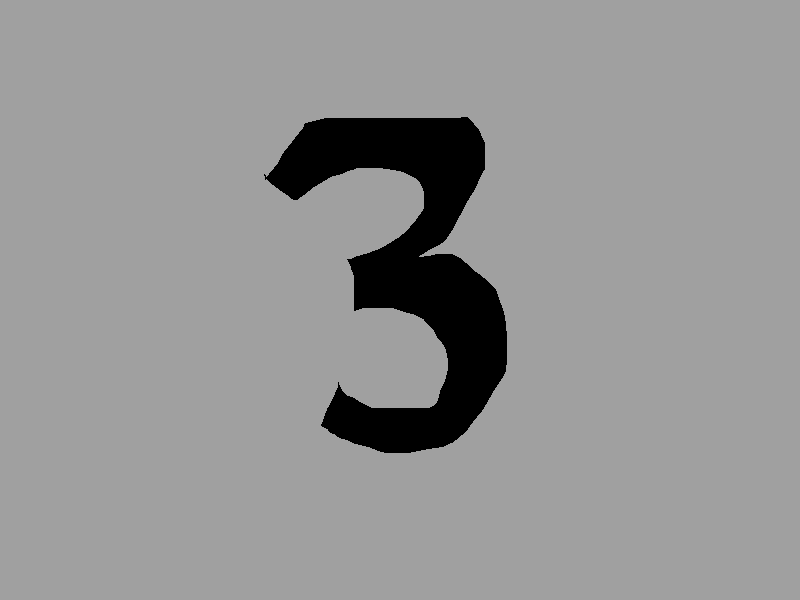
\includegraphics[width=7in,height=4in,keepaspectratio]{images/Image3example.png}};
    \labelnode{2}{2}{3};
\end{tikzpicture}
%\vfill\null
%\pagebreak

% == Closer == 
\label{LastPageRef}
\vfill\null

\end{center}
\end{document}
